%!TEX root = ../report.tex
\begin{document}
\chapter{Methodology}
\label{chapter:methodology}
This chapter will discuss the RandlLA-Net used for 3D semantic segmentation, especially about network architecture and how it helps in better segmentation.
We also discuss the details of the Deep Ensembles and the Flipout methods for uncertainty quantification.
We also study the evaluation metrics for 3D semantic segmentation and OOD detection and the methods to generate OOD scores, such as Maximum Softmax Probability (MSP) as a baseline method and Entropy.
\section{RandLA-Net}
\label{sec:meth_randla}
As stated in \cite{Hu_2020_CVPR_Randla}, it is a lightweight and efficient neural network architecture for semantic segmentation of 3D point clouds.
From Section~\ref{sec:dl_approach}, we can observe that the RandLA-Net architecture is best performing among the point models.
Efficient computation, memory usage and a model with direct application o 3D points are the primary motivation when developing the RandLA-Net.
RandLA-Net employs random point sampling and the local feature aggregation module to achieve these goals.
Authors in \cite{Hu_2020_CVPR_Randla} proved that a successive application of random point sampling along with the local feature aggregation module effective reduce and extracts the features of the large scale point clouds from a scale of $10^5$ to $10^2$.

RandLA-Net utilizes random point sampling among the other sampling methods such as Farthest Point Sampling, Inverse Density Point Sampling.
We select K points uniformly from the original point cloud in random point sampling and have a computational complexity time of O(1).
Random point sampling has the lowest computational complexity and computation time independent of the number of points compared with other point sampling methods.
Despite these advantages, random point sampling has a significant disadvantage of dropping essential points.
To overcome this, the authors of RandLA-Net proposed a local feature aggregation module for the progressive capture of complex features on these selected points.
\begin{figure}
    \centering
    \begin{subfigure}{0.45\textwidth}
        \centering
            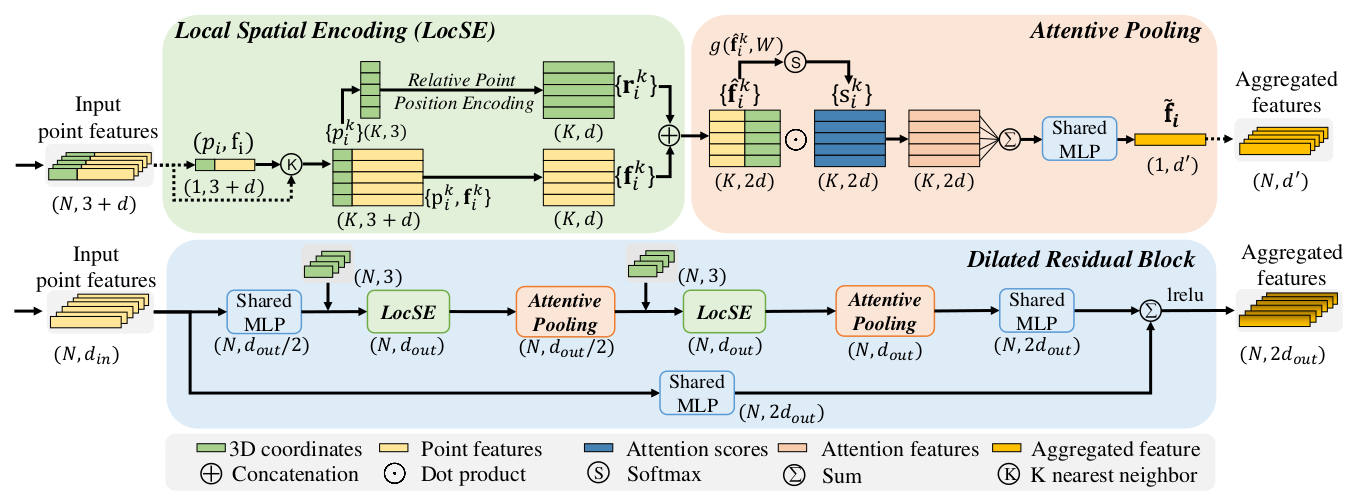
\includegraphics[scale=0.4, angle=90]{images/localfeatueaggregation-randlanet.png}
            \caption{}
            \label{fig:randlanetlfa}       
    \end{subfigure}
    \begin{subfigure}{0.45\textwidth}
        \centering
            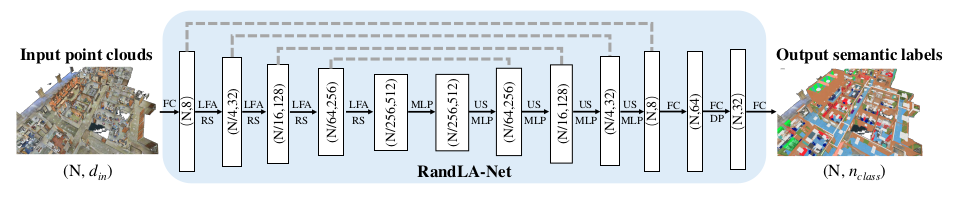
\includegraphics[scale=0.55, angle=90]{images/randlanet.png}
            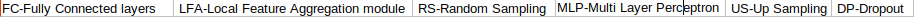
\includegraphics[scale=0.55, angle=90]{images/archi_expl.png}
            \caption{}
            \label{fig:networkarchitecture}
    \end{subfigure}
    \caption{Illustration of (a) local feature aggregation module in RandLa-Net and (b) architecture of RandLA-Net. Both the images are taken from \cite{Hu_2020_CVPR_Randla}.}
\end{figure}

Figure \ref{fig:randlanetlfa} represents the local features aggregation module for the RandLA-Net.
This module is applied parallelly on the 3D points, and the architecture of the local feature aggregation module is further divided into three sub-modules.
They are local spatial encoding (LocSE), attentive pooling and dilated residual blocks represented as green, pink and blue blocks, respectively, in Figure \ref{fig:randlanetlfa}.
Let us discuss further each of these submodules in detail.

\subsection{Local Spatial Encoding (LocSE)}
The local spatial encoding module takes each point ($p_i$) in the point cloud (P) and encodes its neighbouring points' position(x, y and z).
This encoding makes sure that point p always has information about its neighbours.
Also, this encoding helps in learning geometric patterns and learning complex structures progressively.
This module works in three steps:
\begin{enumerate}
    \item Finding nearest neighbours
    \item Relative position encoding
    \item Feature augmentation
\end{enumerate}

In step 1, neighbour points for point ($p_i$) are collected using the euclidean distance-based K-nearest neighbour (KNN) algorithm.
Step 2 encodes these collected K-points for point ($p_i$) using a Multi-Layer Perceptron (MLP) into relative point position. The encoding formula is given by
$$
r_i^k = MLP(p_i \oplus p_i^k \oplus (p_i - p_i^k) \oplus ||p_i-p_i^k||)
$$
where $r_i^k$ is the relative position of point $p_i$ with respect to $p_i^k$, here in $p_i$ and $p_i^k$ only the x,y and z positions are used.
$\oplus$, and $||p_i-p_i^k||$ represents the concatenation operation and euclidean distance calculation between $p_i$ and $p_i^k$ respectively.
This step 2 of relative position encoding is represented by the above part in the LocSE module in the green track in Figure \ref{fig:randlanetlfa}.
Step 3 creates a augmented feature vector $\hat{f_i^k}$ by concatenation of relative point position ($r_i^k$) and its point features ($f_i^k$) of point $p_i^k$.
Point features ($f_i^k$) include the R, G and B values and other features such as intensity values.
This step 3 is represented in the lower part of the LocSE module in the yellow track in Figure \ref{fig:randlanetlfa}.
\subsection{Attentive Pooling}
This augmented feature vector $\hat{f_i^k}$ from the LocSE module is passed through a pooling layer to extract essential features.
Authors state that use of max and mean pooling layer leads to loss of information. Because of this, the authors made use of the attention mechanism, which helps in learning important features automatically.
Given the feature vector, $\hat{f_i^k}$ a function $g$ is learned with the help of MLP and softmax, and the resultant vector is denoted as $s_i^k$ in the pink block in Figure \ref{fig:randlanetlfa}.
These each feature score $s_i^k$ from function $g$ is multiplied with feature vector $f_i^k$ called informative feature vector and summed up to form a unique feature vector $\tilde{f_i}$ for point $p_i$ and this operation is mathematically denoted as
$$
\tilde{f_i}= \sum_{k=1}^K (\hat{f_i^k}.s_i^k)
$$

\subsection{Dilated Residual Block}
Dilated Residual Block is a ResNet inspired module as claimed by authors and represented as a blue colour module in Figure \ref{fig:randlanetlfa}.
This module combines multiple LocSE, Attentive Polling, and a skip connection that feeds an informative feature vector to output.
\begin{figure}
    \centering
    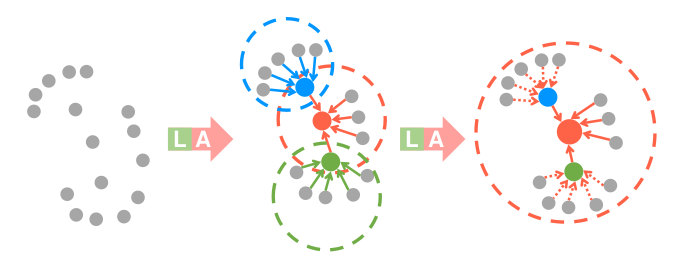
\includegraphics[scale=0.5]{images/dilatedresidualblock.png}
    \caption{Image depicting the working of Dilated residual block with each circle representing the receptive field of the block for feature extraction. Image taken from \cite{Hu_2020_CVPR_Randla}.}
    \label{fig:dilatedresidualblock}
\end{figure}
Let us consider a red point in Figure \ref{fig:dilatedresidualblock}. After applying the first LocSE and Attentive Pooling module, it observes that K neighbours are represented in the red circle.
A secondary application of LocSE and Attentive Polling allows the red point to observe $K^{2}$ neighbours represented as a large red circle in the right subimage in Figure \ref{fig:dilatedresidualblock}.
This progressive dilation of receptive fields allows for observing local features in the first application of LocSe and Attentive Pooling and then observing global features on further application of LocSE and Attentive Polling modules.
Authors claim that the more LocSE and Attentive Pooling stacked in Dilated Residual Block powerful the Dilated Residual Block becomes and greater the receptive field at the expense of computational time.
Authors also claim that only the stacked application of two LocSE and Attentive Pooling modules is powerful enough, and it is effective and efficient in computational time.

To summarize, up to this point, we have studied the unique feature of RandLA-Net. That is how random point sampling in conjecture with local features aggregation module in Figure \ref{fig:randlanetlfa} helps in the extraction of features progressively.
We also studied how the local feature aggregation module is divided into three sub-modules: Local Spatial Encoding (LocSE), Attentive Pooling and Dilated Residual Block. Each of these submodules' working procedures.
In the next section, we study the architecture of RandLA-Net.

\subsection{RandLA-Net architecture}
RandLA-Net is an encoder-decoder architecture with skip connections as used in various segmentation networks such as 3D U-Net\cite{wang2018two_3DUnet}.
The input point clouds are directly applied to the encoder consisting of Fully Connected (FC) and four Local Feature Aggregation (LFA) modules connected sequentially.
The point cloud size reduces by four for every encoder layer. 
Similarly, four decoder layers are used, and the input features maps to each decoder layer are upsampled and concatenated to respective encoder feature maps via skip connections.
The MLP is applied and fed into the next decoder layer.
The output of the final decoder layer is fed into three FC layers for point classification, and a dropout layer is added before the last layer with a dropout rate of 0.5.
The detailed network architecture is illustrated in Figure \ref{fig:networkarchitecture}.

We chose RandLA-Net because of the following reasons:
\begin{enumerate}
    \item Efficient extraction of complex structures progressively using Local Feature Aggregation (LFA) module.
    \item Has fewer parameters (1.24M), making training efficient, as 3D semantic segmentation models are computationally expensive.
    \item Proven performance over a variety of datasets such as Semantic3D and SemanticKITTI, along with ablation study of each submodule in LFA proposed in \cite{Hu_2020_CVPR_Randla}.
    \item No preprocessing such as range image representation as in \cite{Milioto2019}, or farthest point sampling with a computational complexity of $O(N^2)$ as in \cite{Qi_2017_CVPR_pointnet}. Whereas RandLA-Net employs random point sampling with a computational time of $O(1)$.
    \item State of the art performance in point-based methods, consisting of only Multi-Layer Perceptrons (MLP) and without expensive operations such as kernelization or graph construction.
\end{enumerate}

\subsection{Evaluation metrics-Semantic Segmentation}
To evaluate the performance of RandLA-Net over the training dataset (Semantic3D in our case), we chose two metrics.
They are Mean Intersection-over-Union (mIoU) and Accuracy.

\subsubsection{Mean Intersection-over-Union (mIoU)}
Mean Intersection-over-Union is a widely used metric for performance evaluation in the task of semantic segmentation.
It is calculated as a mean of a fraction of the intersection area between predicted and ground-truth masks and the union of predicted and ground truth masks.
mIoU is calculated as
$$mIoU=\frac{1}{N}\sum_{k=1}^N \frac{p_k\cap g_k}{p_k \cup g_k}$$
Where $N$ is the number of classes, $p_k$ and $g_k$ are predicted mask and ground truth mask of $k^{th}$ class.

\subsubsection{Accuracy}
Accuracy is another widely used metric, which can be quantified as a number of points in the point cloud correctly classified.
It can be formulated from the confusion matrix as
$$Accuracy = \frac{TP+TN}{TP+TN+FP+FN}$$
Where TP, TN, FP and FN are True Positives, True Negatives, False Positives and False Negatives, respectively, from the confusion matrix.
This metric alone can be misleading in case of severe class imbalance.

Here, we conclude the study of RandLA-Net, the reason for its effective performance, argue the reasons to chose RandLA-Net and briefly discuss the evaluation metrics used.
In the following sections, we will discuss the utilized uncertainty estimation methods such as deep ensembles, Flipout and metrics used to evaluate 3D semantic segmentation and OOD detection.
\section{Deep ensembles}
\label{sec:meth_deepensembles}
Deep ensembles employ a kind of ensemble learning technique and are proposed in \cite{lakshminarayanan2016simple}.
Like bagging, the idea is to train the same network with the same data with random initializations N number of times.
These N trained models converge similarly with little difference given the same training conditions and hyperparameters.
\begin{figure}
    \centering
    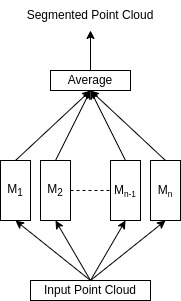
\includegraphics[scale=0.55]{images/DE.jpg}
    \caption{Illustration of test dataflow in Deep Ensembles, where input point cloud is fed into multiple randomly initialized models ($M_1-M_n$). 
    These individual predictions from each model are averaged to compute the final prediction.}
    \label{fig:deepensembles}
\end{figure}
An example of a deep ensemble is depicted in Figure \ref{fig:deepensembles}.
Here the input point cloud is fed into N number of models. In our case, these models are all RandLA-Net.
The resulting predictions are combined to get the final prediction. 
The combination is done by averaging over all the predictions of N models to get the final predictions in our case.
Deep ensembles are proven to improve the overall performance of the model as in \cite{bhandary2020evaluating}, and we also expect the same behaviour in our case.

Despite their performance boosting ability, they are also used to estimate uncertainty as in \cite{lakshminarayanan2016simple}.
\cite{lakshminarayanan2016simple} proposes that with the increase in the number of ensembles, the Negative Log-Likelihood (NLL) and Brier score goes down, suggesting the network produces well-calibrated predictions.
\cite{lakshminarayanan2016simple} also studies the effect of entropy with out-of-distribution (OOD) classes.
They performed the study on MNIST-NotMNIST and SVHN-CIFAR10, with the first dataset in pair being in distribution (ID) and the second dataset being the OOD dataset.
The authors verified that entropy distribution on the ID dataset is peaky. Similarly, the entropy distribution on the OOD dataset is more spread across all entropy values.
We hypothesize that similar performance is observed in 3D semantic segmentation as a task of segmentation can be treated as multi-class classification in a point cloud.
Because proven ability to classify OOD on the classification task boosts the model's performance and ease of implementation makes deep ensembles an ideal candidate for OOD detection in 3D semantic segmentation.

\section{Flipout}
\label{sec:meth_flipout}
In this thesis, we also employed the Flipout version of the RandLA-Net model for uncertainty estimates, and in this section, we discuss Flipout and its application.
Flipout has initially been introduced in \cite{Flipout} as an efficient method of gradient decorrelation in a mini-batch of examples.
This effect is implemented by adding independent weight perturbations sampled from distribution for each example.
Authors in \cite{Flipout} describe weight perturbations as methods whose weights of the neural network are sampled from distribution during training.
In general, neural network weights are point estimates where the weight is a single scalar value. In the case of weight perturbations, they are modelled as a distribution where each weight $W=\overline{W}+\Delta W$ in which $\overline{W}$ is the mean weight and $\Delta W$ is the perturbation.
If this $\Delta W$ is sampled from a Gaussian distribution, it is called a Gaussian perturbation.
Since the sampled weight perturbation is the same for all the examples over the mini-batch, the authors argue a correlation between the gradients.
So authors of Flipout make two critical assumptions to deal with this problem. 
They are a perturbation of different weights should be different, and the distribution of perturbation should be symmetric around zero.
So under these assumptions, the authors observed that the perturbation distribution is invariant to element-wise multiplication of the random sign matrix.
Here random sign matrix is defined as a matrix whose elements are randomly sampled uniformly from $\pm 1$. 
So the weight perturbation is modelled as Equation~\ref{eq:flipout_main} where $\widehat{\Delta W}$ is the base perturbation which is same for all weights, $\times$ represents element wise multiplication, $r_n, s_n$ represent the randomly signed vectors of ($\pm 1$) and $\Delta W_n$ is the perturbation of $n^{th}$ weight.
\begin{equation}
    \Delta W_n = \widehat{\Delta W} \times r_n s_{n}^T
    \label{eq:flipout_main}
\end{equation}
So the node output of the neural network is modified as 
$$y_n = \phi(W^T x_n) $$
$$y_n = \phi((\overline{W}+\widehat{\Delta W} \times r_n s_{n}^T)^Tx_n)$$
$$y_n = \phi(\overline{W} x_n+(\widehat{\Delta W}^T (x_n\times s_{n}))\times r_n)$$
Here $\phi$ is the activation function, and $x_n$ is the $n^{th}$ input example in the mini batch.
This whole operation is vectorized and is stated as a matrix multiplication in Equation~\ref{eq:fowpass_flipout} where $R$ and $S$ consist of rows of $r_n$ and $s_n$.
Here $R$ and $S$ are independent of $\overline{W}$ and $\widehat{\Delta W}$ which does not add any additional terms in backpropagation.
\begin{equation}
    Y = \phi(X\overline{W}+((X\times S)\widehat{\Delta W})\times R)
    \label{eq:fowpass_flipout}
\end{equation}
Authors also argue that the Flipout reduces the variance in gradients when compared to shared perturbation but has a slightly higher variance than independent perturbations along with the mathematical proof produced in \cite{Flipout}.


At a glance, these random weight perturbations give us slightly different output estimates for every forward pass.
In our case, we changed the few classification layers of the network to Flipout compatible more about the setup in Section \ref{sec:flipout_setup}.
We then compute the forward pass multiple times, and these multiple output estimates from multiple forward passes are then averaged to get the final prediction estimate.
A representation of this operation is presented in Figure~\ref{fig:flipout_ex}, and here, $F_1$ represents the single feature extraction network, and these features are fed into multiple classification heads represented from $C_1$ to $C_N$.
These classifications are averaged to get the final classification score.

\begin{figure}
    \centering
    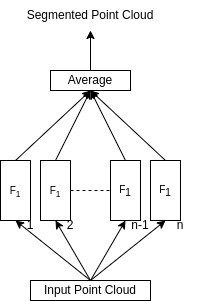
\includegraphics[scale=0.5]{images/flipout.jpg}
    \caption{Illustration of test dataflow in Flipout. Here $F_1$ represents the flipout trained model and we compute n forward passes of the same point cloud on $F_1$.
    These individual predictions are averaged to compute the final predictions.}
    \label{fig:flipout_ex}
\end{figure}
\FloatBarrier

\section{OOD estimates}
In this section, we discuss the two methods used to generate the OOD score for classifying the OOD objects and how these scores are calculated.
The two metrics are Maximum Softmax Probability (MSP) and Entropy.

\subsection{Maximum Softmax Probability}
First proposed in \cite{hendrycks2016baseline_MSP}, uses the probability of the classification from the Softmax for OOD detection. 
MSP still serves as the most evaluated baseline method for OOD detection.
Since we are the first study to perform OOD detection 3D semantic segmentation to the best of our knowledge, we wanted to incorporate this score as a baseline. 
Here the main idea is that if a point in a point cloud is known, then it will have a higher MSP score and vice versa.
It is calculated as a given in Equation~\ref{eq:MSP_formula}, where $y_n$ is the list of softmax probablity score for each class given as $p_1, p_2, .., p_n$.
$$y_n = [p_1, p_2,..,p_n]$$
\begin{equation}
    MSP = max(y_n)
    \label{eq:MSP_formula}
\end{equation}

\subsection{Entropy}
\label{sec:meth_entropy}
Entropy is defined by \cite{entropy_robinson} as an "ill-defined notion of chaos or uncertainty".
Entropy has its roots in thermodynamics, and in computer science, it can be used as a measure of information content.
In deep learning, Entropy is used as a measure for uncertainty and calculated as given in Equation~\ref{eq:ent_calc}, where $P(x_i)$ is softmax probablity for $i^{th}$ of point x.
\begin{equation}
    Entropy = -\sum_i P(x_i) log P(x_i)
    \label{eq:ent_calc}
\end{equation}
In theory, following this formula, if the point in the point cloud is from In Distribution (ID), the softmax output is higher for one class, and other classes will be near zero.
This leads to a lower entropy score for the ID point, and for the Out Of Distribution (OOD) point in the point cloud, the softmax output is spread across all the classes.
This means that the OOD point will have a higher entropy score.

\section{Evaluation metric-OOD detection}
This section will discuss the metrics used for evaluating OOD detection. Firstly the Receiver Operating Characteristic (ROC) curve to extract thresholds of the score and later the Area Under the ROC curve (AUROC) for evaluation and comparison of the OOD detection performance.
\subsection{Receiver Operating Characteristic Curve}
ROC curves are typically used for selecting the best classifiers based on their performance.
ROC curves were historically used in signal detection but later found their way into the machine learning community.
According to \cite{ROC_example}, this is because accuracy itself is a poor metric to realise the model's performance.
Also, ROC curves are insusceptible to change in class distribution, that is, the proportion of negative to positive examples.
ROC curves are drawn based on True Positive Rate (TPR) and False Positive Rate (FPR).
TPR is calculated as the number of positively classified samples to the total positive samples. FPR is calculated as the number of negatively classified samples to the total number of negative samples.

A ROC curve is generated, given a set of probabilities/scores and their true labels, either positive or negative.
We then generate a range of threshold values from these probabilities and compute TPR and FPR for each threshold value.
These TPR and FPR are plotted to generate a ROC curve as displayed in Figure~\ref{fig:ROC_curve_example}. 
Figure~\ref{fig:ROC_curve_example} represents ROC curves for various classifiers, and here red line represents the roc curve for the random classifier. The green line represents the roc curve for a perfect classifier.
Since we want our classifier to perform better than a random classifier, we expect our ROC curve to be in the blue region.
\begin{figure}[!ht]
    \centering
    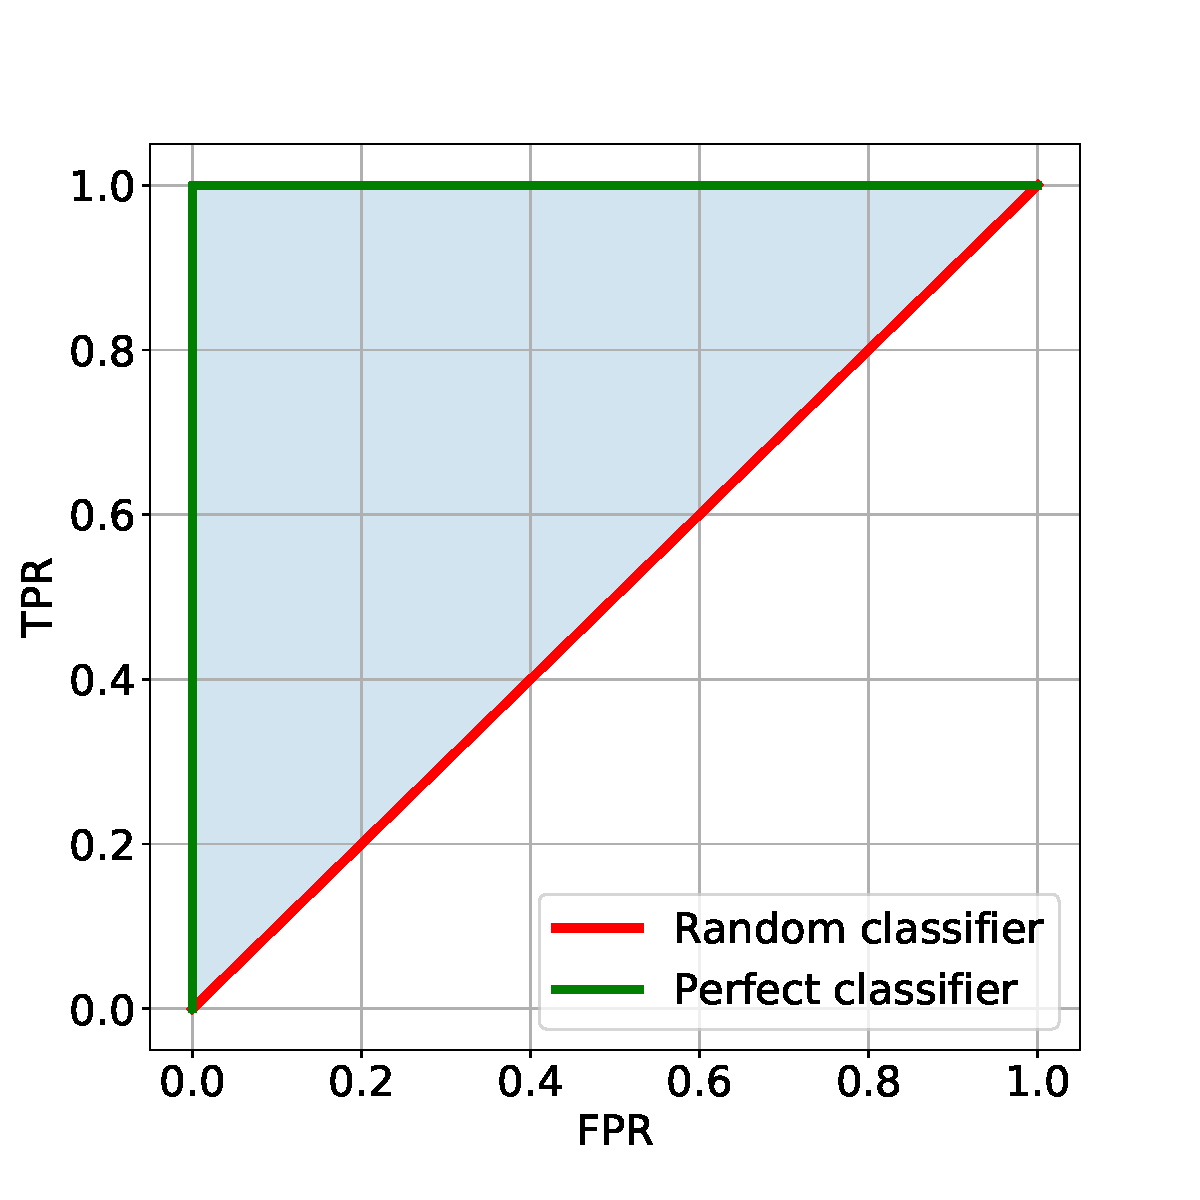
\includegraphics[scale=0.35]{images/ROC_curve_example.pdf}
    \caption{Illustration of example ROC curves with red curve for random classifier and green curve representing the perfect classifier.
    Our classifier ROC curve is expected to be placed in this blue shaded region.}
    \label{fig:ROC_curve_example}
\end{figure}

\subsection{Area Under an ROC curve}
Since the ROC curves are a tow dimensional depiction and we need a single scalar value to compare the performance of the classifiers, we use the Area Under a ROC curve (AUROC) value.
AUROC is the area enclosed below the ROC curve, and the AUROC value ranges between 0 and 1 as the curve is plotted in a unit square.
AUROC for a random classifier's ROC curve as depicted in red colour in Figure~\ref{fig:ROC_curve_example} is 0.5, and the perfect classifier depicted as the green line is one as its area encompasses the whole square.
In this thesis, we use this score to evaluate and compare the performance of OOD detection between Deep Ensembles and Flipout.

\end{document}
